%%%%%%%%%%%%%%%%%%%%%%%%%%%%%%%%%%%%%%%%%
% Programming/Coding Assignment
% LaTeX Template
%
% This template has been downloaded from:
% http://www.latextemplates.com
%
% Original author:
% Ted Pavlic (http://www.tedpavlic.com)
%
% Note:
% The \lipsum[#] commands throughout this template generate dummy text
% to fill the template out. These commands should all be removed when 
% writing assignment content.
%
% This template uses a Perl script as an example snippet of code, most other
% languages are also usable. Configure them in the "CODE INCLUSION 
% CONFIGURATION" section.
%
%%%%%%%%%%%%%%%%%%%%%%%%%%%%%%%%%%%%%%%%%

%----------------------------------------------------------------------------------------
%	PACKAGES AND OTHER DOCUMENT CONFIGURATIONS
%----------------------------------------------------------------------------------------

\documentclass[a4paper]{article}

\usepackage{fancyhdr} % Required for custom headers
\usepackage{lastpage} % Required to determine the last page for the footer
\usepackage{extramarks} % Required for headers and footers
\usepackage[usenames,dvipsnames]{color} % Required for custom colors
\usepackage{graphicx} % Required to insert images
\usepackage{listings} % Required for insertion of code
\renewcommand*{\lstlistingname}{代码} % change "Listing <ref> to 代码 <ref>
\usepackage{courier} % Required for the courier font
\usepackage{lipsum} % Used for inserting dummy 'Lorem ipsum' text into the template

\usepackage[UTF8]{ctex} % Required for Chinese character
\usepackage{tocloft} % Required for beautiful toc
\usepackage[hidelinks]{hyperref} % Required for clickable toc
\hypersetup{
    colorlinks,
    citecolor=black,
    filecolor=black,
    linkcolor=black,
    urlcolor=black
}
\usepackage[title]{appendix} % Required for appendix
\usepackage{float}
\usepackage{amsmath} % used for \text{} in math formula


% used for beautiful table
\usepackage{booktabs} 
\usepackage[T1]{fontenc}
\usepackage{tabu}
\usepackage{longtable}
\usepackage[table]{xcolor}


% Margins
\topmargin=-0.45in
\evensidemargin=0in
\oddsidemargin=0in
\textwidth=6.5in
\textheight=9.0in
\headsep=0.25in

\linespread{1.1} % Line spacing

% Set up the header and footer
\pagestyle{fancy}
\lhead{\hmwkAuthorName} % Top left header
\chead{\hmwkClass\ (\hmwkClassInstructor\ \hmwkClassTime): \hmwkTitle} % Top center head
\rhead{\firstxmark} % Top right header
\lfoot{\lastxmark} % Bottom left footer
\cfoot{} % Bottom center footer
\rfoot{Page\ \thepage\ of\ \protect\pageref{LastPage}} % Bottom right footer
\renewcommand\headrulewidth{0.4pt} % Size of the header rule
\renewcommand\footrulewidth{0.4pt} % Size of the footer rule

\setlength\parindent{0pt} % Removes all indentation from paragraphs

%----------------------------------------------------------------------------------------
%	CODE INCLUSION CONFIGURATION
%----------------------------------------------------------------------------------------

\definecolor{MyDarkGreen}{rgb}{0.0,0.4,0.0} % This is the color used for comments
\lstloadlanguages{c} % Load Perl syntax for listings, for a list of other languages supported see: ftp://ftp.tex.ac.uk/tex-archive/macros/latex/contrib/listings/listings.pdf
\lstset{language=c, % Use Perl in this example
        frame=single, % Single frame around code
        basicstyle=\small\ttfamily, % Use small true type font
        keywordstyle=[1]\color{Blue}\bf, % Perl functions bold and blue
        keywordstyle=[2]\color{Purple}, % Perl function arguments purple
        keywordstyle=[3]\color{Blue}\underbar, % Custom functions underlined and blue
        identifierstyle=, % Nothing special about identifiers                                         
        commentstyle=\usefont{T1}{pcr}{m}{sl}\color{MyDarkGreen}\small, % Comments small dark green courier font
        stringstyle=\color{Purple}, % Strings are purple
        showstringspaces=false, % Don't put marks in string spaces
        tabsize=4, % 5 spaces per tab
        %
        % Put standard Perl functions not included in the default language here
        % morekeywords={rand},
        morekeywords = [1]{uint16_t, uint32_t, uint8_t, int16_t, int8_t, int32_t}
        %
        % Put Perl function parameters here
        morekeywords=[2]{on, off, interp, __attribute__},
        %
        % Put user defined functions here
        morekeywords=[3]{test},
       	%
        morecomment=[l][\color{Blue}]{...}, % Line continuation (...) like blue comment
        numbers=left, % Line numbers on left
        firstnumber=1, % Line numbers start with line 1
        numberstyle=\tiny\color{Blue}, % Line numbers are blue and small
        stepnumber=2, % Line numbers go in steps of 5,
        firstnumber=1
}

% define C style
\definecolor{main-color}{rgb}{0.6627, 0.7176, 0.7764}
\definecolor{back-color}{rgb}{0.1686, 0.1686, 0.1686}
\definecolor{string-color}{rgb}{0.3333, 0.5254, 0.345}
\definecolor{key-color}{rgb}{0.8, 0.47, 0.196}
\lstdefinestyle{mystyle}
{
    language = C++,
    basicstyle = {\small\ttfamily},
    stringstyle = {\color{Mahogany}},
    keywordstyle = {\color{blue}},
    keywordstyle = [2]{\color{Mahogany}},
    keywordstyle = [3]{\color{blue}},
    keywordstyle = [4]{\color{blue}},
    otherkeywords = {__attribute__,<<,>>,++},
    morekeywords = [2]{__attribute__},
    morekeywords = [3]{<<, >>},
    morekeywords = [4]{++, uint16_t, uint32_t, uint8_t, \#define},
}


% Creates a new command to include a perl script, the first parameter is the filename of the script (without .pl), the second parameter is the caption

\newcommand{\shfilescript}[3]{
\begin{itemize}
\item[]\lstinputlisting[caption=#2, label=lst:#1, language=sh]{#3}
\end{itemize}
}
\newcommand{\shscript}[3]{
\begin{itemize}
\item[]\begin{lstlisting}[label=lst:#1, caption=#2] #3 \end{lstlisting}
\end{itemize}
}

%----------------------------------------------------------------------------------------
%	DOCUMENT STRUCTURE COMMANDS
%	Skip this unless you know what you're doing
%----------------------------------------------------------------------------------------

% Header and footer for when a page split occurs within a problem environment
\newcommand{\enterProblemHeader}[1]{
\nobreak\extramarks{#1}{#1 见下页\ldots}\nobreak{} 
\nobreak\extramarks{接上页}{#1 见下页\ldots}\nobreak{}
}

% Header and footer for when a page split occurs between problem environments
\newcommand{\exitProblemHeader}[1]{
\nobreak\extramarks{接上页}{#1 见下页\ldots}\nobreak{}
\nobreak\extramarks{#1}{}\nobreak{}
}
% TODO:code here enable the number before section, but it disable the numbering of problems
%\setcounter{secnumdepth}{0} % Removes default section numbers
\newcounter{homeworkProblemCounter} % Creates a counter to keep track of the number of problems

\newcommand{\homeworkProblemName}{}

\newenvironment{homeworkProblem}[1][Problem \arabic{homeworkProblemCounter}]{ % Makes a new environment called homeworkProblem which takes 1 argument (custom name) but the default is "Problem #"
\stepcounter{homeworkProblemCounter} % Increase counter for number of problems
\renewcommand{\homeworkProblemName}{#1} % Assign \homeworkProblemName the name of the problem
\section{\homeworkProblemName} % Make a section in the document with the custom problem count
\enterProblemHeader{\homeworkProblemName} % Header and footer within the environment
}{
\exitProblemHeader{\homeworkProblemName} % Header and footer after the environment
}

\newcommand{\problemAnswer}[1]{ % Defines the problem answer command with the content as the only argument
\noindent\framebox[\columnwidth][c]{\begin{minipage}{0.98\columnwidth}#1\end{minipage}} % Makes the box around the problem answer and puts the content inside
}

\newcommand{\homeworkSectionName}{}
\newenvironment{homeworkSection}[1]{ % New environment for sections within homework problems, takes 1 argument - the name of the section
\renewcommand{\homeworkSectionName}{#1} % Assign \homeworkSectionName to the name of the section from the environment argument
\subsection{\homeworkSectionName} % Make a subsection with the custom name of the subsection
\enterProblemHeader{\homeworkProblemName\ [\homeworkSectionName]} % Header and footer within the environment
}{
\enterProblemHeader{\homeworkProblemName} % Header and footer after the environment
}


\newcommand{\codev}[1]{\textsf{#1}}
%----------------------------------------------------------------------------------------
%	NAME AND CLASS SECTION
%----------------------------------------------------------------------------------------

% table color
\definecolor{tableHeader}{RGB}{245, 245, 245}
\definecolor{tableLineOne}{RGB}{245, 245, 245}
\definecolor{tableLineTwo}{RGB}{224, 224, 224}
\newcommand{\tableHeaderStyle}{
    \rowfont{\leavevmode\color{white}\bfseries}
    \rowcolor{tableHeader}
}

%----------------------------------------------------------------------------------------

\newcommand{\hmwkTitle}{操作系统原理实验\ \#6} % Assignment title
\newcommand{\hmwkDueDate}{Saturday,\ April\ 28,\ 2018} % Due date
\newcommand{\hmwkClass}{16级计科\ 7班} % Course/class
\newcommand{\hmwkClassTime}{周一9-10节} % Class/lecture time
\newcommand{\hmwkClassInstructor}{凌应标} % Teacher/lecturer
\newcommand{\hmwkAuthorName}{颜彬} % Your name
\newcommand{\hmwkAuthorId}{16337269} % Your id 

%----------------------------------------------------------------------------------------
%	TITLE PAGE
%----------------------------------------------------------------------------------------

\usepackage{titling}

\title{
\vspace{2in}
\textmd{\textbf{\hmwkClass:\ \hmwkTitle}}\\
\normalsize\vspace{0.1in}\small{Due\ on\ \hmwkDueDate}\\
\vspace{0.1in}\large{\textit{\hmwkClassInstructor\ \hmwkClassTime}}
\vspace{3in}
}

\author{\textbf{\LARGE{\hmwkAuthorName}} \\ \\ \textbf{\LARGE{\hmwkAuthorId}}}
\date{} % Insert date here if you want it to appear below your name
%----------------------------------------------------------------------------------------

\begin{document}
% \begin{titlingpage} % This is for ignore page number in first page. package titling

\maketitle

%----------------------------------------------------------------------------------------
%	TABLE OF CONTENTS
%----------------------------------------------------------------------------------------

% \setcounter{tocdepth}{2} % Uncomment this line if you don't want subsections listed in the ToC
% set depth in toc

% \renewcommand{\cftsecleader}{\cftdotfill{\cftdotsep}} % used for dots between <section> and <page>

\renewcommand{\contentsname}{Content} % force the word to be "content
\newpage
\tableofcontents
\addtocontents{toc}{~\hfill\textbf{Page}\par}
\newpage

% below are document body


% To have just one problem per page, simply put a \clearpage after each problem
\section{实验目的}
理解多道程序和分时系统的实现原理。理解二进程模型的原理。熟悉进程调度的方法。
理解并能自行设计进程控制块,存储必要的进程信息。设计进程表和相关底层函数
接口供内核调用。进一了解时钟中断的工作原理,完成用户程序的轮流执行。
\section{实验过程}
    \subsection{进程控制块}
    进程控制块中最核心的部分是寄存器映像RegisterImage.其实现如代码\ref{lst:PCB}所示。
    整个寄存器映像可以分为若干个部分。\\ 

    第一个部分是flags, cs和ip。它在中断发生时自动入栈。\\ 

    第二部分是ax, cs, dx, bx, sp, bp, si, di。这部分可以由pusha指令推入栈中。结构体中
    这些寄存器的排列顺序恰好是pusha指令入栈的顺序。根据文档,pusha压入栈中的sp是
    ``执行pusha前的sp的值''。在结构体中,该sp称为``old\_sp''。(与以后提到的``sp''相区分)
    值得一提的是该C语言编译时必须关闭所有优化,否则
    编译器可能会进行重排操作。\\ 

    第三个部分是段寄存器,从ds到ss。这部分在保护现场时,用push指令手动入栈。\\ 

    最后一个部分只包含一个寄存器,sp.该sp值的是在把所有的其他寄存器都压入栈中后的sp的值。该值
    在\ref{sec:save}节的现场保护和第\ref{sec:load}节的现场恢复中极其重要。
    \begin{figure}[!hbt]
    \begin{itemize}
    \item[] \begin{lstlisting}[language=C, label=lst:PCB, caption=PCB寄存器映像]
struct RegisterImage {
    uint16_t sp;

    //segments
    uint16_t ss;
    ...
    uint16_t ds;

    // pusha
    uint16_t di;
    uint16_t si;
    uint16_t bp;
    uint16_t old_sp;
    uint16_t bx;
    uint16_t dx;
    uint16_t cx;
    uint16_t ax;

    // pushed by interupt
    uint16_t ip;
    uint16_t cs;
    uint16_t flags;
}__attribute__((packed));
    \end{lstlisting}
    \end{itemize}
    \end{figure}

    \subsection{保存上下文}\label{sec:save}
    保存上下文的代码如代码\ref{lst:save}所示。代码大概分为若干的几个部分(空行隔开)。\\ 

    pusha 和一系列的push <segment> 把寄存器保存在栈中。必须在时钟中断到达后的第一时间保存寄存器。这是因为这些寄存器应该与
    flag, cs, ip连续存放。一旦这些寄存器和flag, cs, ip分隔开后,会对PCB块的保存带来很大的麻烦。\\ 

    只有将所有寄存器都保存到栈后,才能执行 mov es, 0 和 mov ds, 0(本代码仅作示意)的操作。由于需要将sp压入栈中,但push sp
    是有歧义的汇编代码,为了可读性和可维护性,这里采用mov [ss:sp-2], sp的写法(本代码仅作示意)。\\ 

    寄存器都保存完毕后,采用rep movsb指令将栈中保存的所有内容复制到PCB块中。
\begin{figure}
\begin{itemize}
\item[] \begin{lstlisting}[language={[x86masm]Assembler}, label=lst:save, caption=保存上下文的实现]
saveRegisterImage:
    ; 高地址
    pusha

    push ds ; sp + 8
    push es ; sp + 6
    push fs ; sp +4
    push gs ; sp + 2
    push ss ; sp 
    ; 低地址
    
    mov ax, 0 ; cs is 0
    mov es, ax
    mov ds, ax

    calll get_current_PCB_address

    mov bx, sp 
    mov word [ss:bx-2], sp 

    mov di, ax
    mov ax, sp
    sub ax, 2
    mov si, ax

    mov cx, 17 * 2
    cld
    rep movsb
\end{lstlisting}
\end{itemize}
\end{figure}
    \subsection{恢复上下文}\label{sec:load}
    恢复现场是保护现场的逆过程。这里采用略为讨巧的方法。恢复现场时,先恢复sp和ss,让栈指针指向``被恢复进程''的栈顶。随后,只需要按照``保存上下文的逆序''
    执行pop指令。即可顺利地恢复所有寄存器的值。随后采用iret,再把flag, cs, ip出栈的同时,把cs和ip恢复到正确的值.\\ 

    这里有若干细节需要注意。首先是,popa指令不会修改sp的值(但它会把sp从栈中弹出)。popa的这个行为很好理解,因为随意修改sp会导致极其严重的错误。(虽然
    在进程切换时,我会更希望popa指令能帮我把sp也修改了)。第二个细节是,无论如何都要先把PCB中的值复制到栈上(哪怕栈上已经有一份一模一样的副本),再做
    进程恢复。这是因为,整个操作系统的第一个进程(INIT进程)需要靠``恢复上下文''操作来自动启动。而第一个进程(INIT进程)的初始化操作是在PCB上做的,而不是
    栈上做的。
    \subsection{内存分配模型}
    本次项目还做了简单的内存分配,支持在内核上对某个保留内存空间的malloc 和free的操作。这允许了用户程序在运行前才分配和指定内存空间。配合项目4完成的
    文件系统,本次项目能更自由和智能地执行用户程序。\\ 

    内存分配器采用若干个链表来实现。首先将0x10000到0x20000的内存空间分成大小为0x20, 0x800, 0x1000的块。这些块组成3个独立的链表。
    每次分配内存时,先计算出最合适的块,从将该块从链表中移除,并返回该块的首地址。在回收内存时,只需将该内存块回收入链表中即可。在经典的
    内存池实现中,内存块的大小应包括4, 8, 16, ..., $2^n$, ..., 1024字节。如此,维护9个独立的链表。本实现简化了这些细节(考虑到项目时间问题),
    仅提供了3种不同大小的块。\\ 

    内存分配需要做初始化。初始化函数如代码\ref{lst:mm_init}所示。代码只截取了有代表性的部分。\\ 

    初始化中,``强行''将内存p中的值修改为p + offset,然后把p修改为p + offset,不断重复以上步骤。如此即可在内存空间中``强行''
    构造出一个链表。\\ 

    在内存分配时,通过将phead = *phead这一操作,将头指针的值改为头指针指向的内存空间的值(下一个块的地址)。如此即可实现将块弹出链表的操作。
    内存回收的代码如\ref{lst:mm_free}所示。若返回的内存块大小大于最大的块,则说明程序出错,直接返回。否则,找到该块属于哪个链表,
    通过两行语句将回收的内存放回到链表的头。在下一次内存申请时,回收的内存可以被再次使用。\\ 
    
    内存分配的示意图如图\ref{fig:mm}所示。其中白色空心箭头(带有HEAD字样)的为内存分配器的头指针。白色空心箭头(带有RETUREN字样)
    的为malloc函数的返回值。内存回收的示意图如\ref{fig:mm_free}所示。其中标号为x的block代表待回收的代码块。\\ 

    由于本次项目时间紧迫。所以没有将malloc和free封装成系统调用。这就导致了分配0x10000~0x20000空间时,段还处在0x0000处。而访问
    0x10000会因为偏移量过大而导致访问错误。所以此处采用了一个变通方案。在进入所有的内存分配器函数之后,先手动把ds置为0x1000.在离开后
    手动恢复ds。如此即可暂时解决这个跨段修改内存的问题。在以后的版本中,会把内存分配封装成系统调用。
    
    \begin{figure}[!hbt]
    \begin{minipage}{0.48\textwidth}
        \centering
        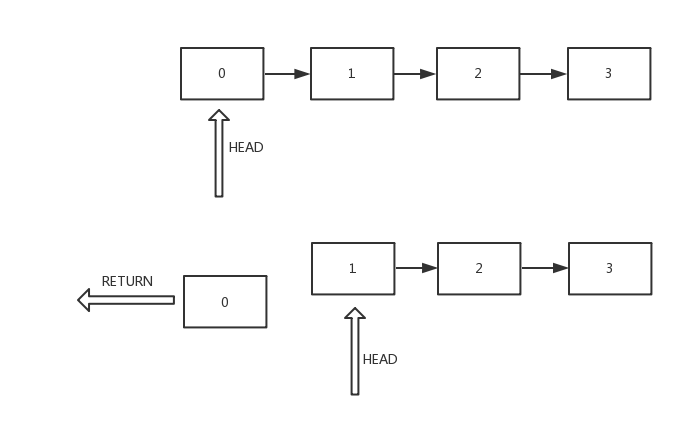
\includegraphics[width=\linewidth]{assets/mm.png}
    \caption{分配内存示意图} \label{fig:mm}
    \end{minipage}\hfill
    \begin{minipage}{0.48\textwidth}
        \centering
        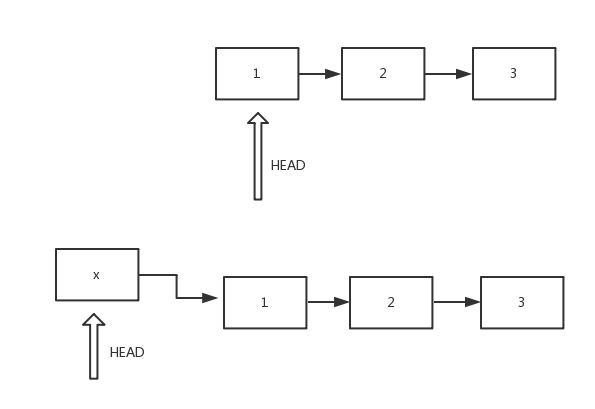
\includegraphics[width=\linewidth]{assets/mm_free.png}
    \caption{内存释放示意图} \label{fig:mm_free}
    \end{minipage}
    \end{figure}
    \begin{figure}
    \begin{itemize}
    \item[] \begin{lstlisting}[language=C, label=lst:mm_init, caption=内存分配器的初始化]
void init_mm() {
    __mm__enter();

    MM_LITTLE_HEAD = (uint32_t*)LITTLE_BEGIN;

    int i = 0;
    void* p = (void* )(LITTLE_BEGIN);
    while (p + BLOCK_LITTLE_SIZE * i <= (void*)LITTLE_END) {
        *(uint32_t*) (p + BLOCK_LITTLE_SIZE * i) 
            = (uint32_t)(p + BLOCK_LITTLE_SIZE * (i+1));
        i++;
    }

    ...

    __mm__leave();
}
    \end{lstlisting}
    \end{itemize}
    \end{figure}

\begin{figure}
\begin{itemize}
\item[] \begin{lstlisting}[language=C, label=lst:mm_free, caption=内存分配器的free操作实现]
void mm_free(uint32_t addr, int32_t size) {
    __mm__enter();
    if (size >= BLOCK_LARGE_SIZE) return;
    else if (size > BLOCK_MID_SIZE) {
        *(uint32_t*)addr = (uint32_t)MM_LARGE_HEAD;
        MM_LARGE_HEAD = (uint32_t*)addr;
    } 
    
    ...

    __mm__leave();
}
\end{lstlisting}
\end{itemize}
\end{figure}
\section{实验结果}
    在进入程序后,输入run stoneQ,或run stoneW,或 run stoneA 或 run stoneS即可在屏幕的4个不同的位置运行stone程序。每次
    新程序运行时,会先调用内存分配器获得分配的内存,初始化进程控制块,并开始进程的执行。

    如图\ref{fig:3_stoneS}所示,进入程序后连续输入3次run stoneQ。随后输入pc指令查看当前线程的状态。可以看到屏幕右下角有3个不同
    的字母'A'在独立地运动(\textbf{图片效果不好,请自行尝试})。同时可以看到这3个不同的进程有自己独立的进程id和内存地址。由于中断占据了0号进程,
    所以这3个用户进程的id为1-3.\\ 

    如图\ref{fig:kp}紧接着上图,继续执行kill 1,把1号进程杀死,并执行run stoneW,产生一个新的stone程序。
    在杀死了1进程后,内存管理器会回收掉进程1占据的内存。在产生新进程时,可以把回收的内存重新分配出去。所以如图所示,
    进程4的内存起始地址为0x11000,恰好为原来进程1的内存地址。\\ 

    图\ref{fig:null}用于证明,本次实验中系统调用仍能正常进行。
    
    \begin{figure}
    \begin{minipage}{0.48\textwidth}
        \centering
        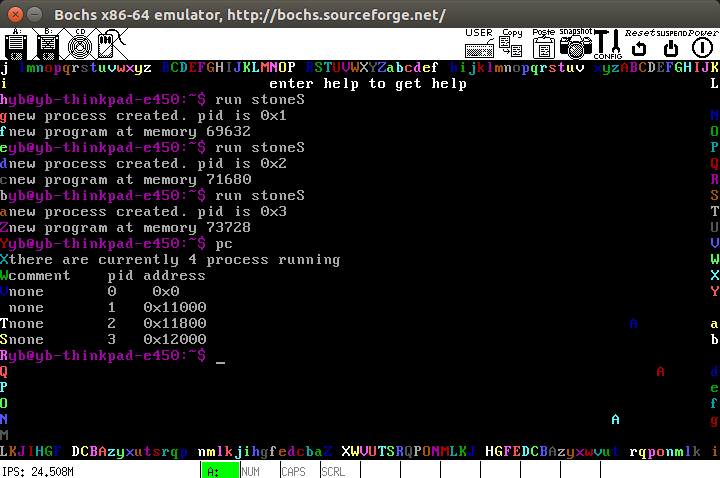
\includegraphics[width=\linewidth]{assets/three_stone_S.png}
    \caption{同时运行3个stoneQ程序的画面} \label{fig:3_stoneS}
    \end{minipage}\hfill
    \begin{minipage}{0.48\textwidth}
        \centering
        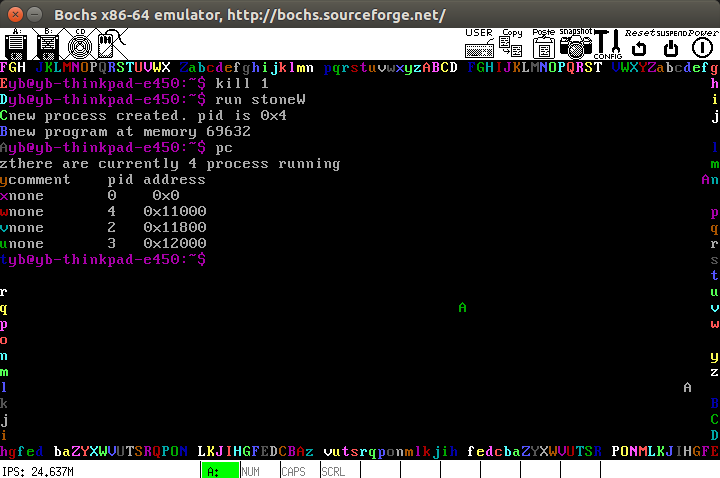
\includegraphics[width=\linewidth]{assets/kill_p.png}
    \caption{杀死一个进程,又创建一个新进程后的画面} \label{fig:kp}
    \end{minipage}
    \end{figure}
    
    \begin{figure}
        \begin{center}
        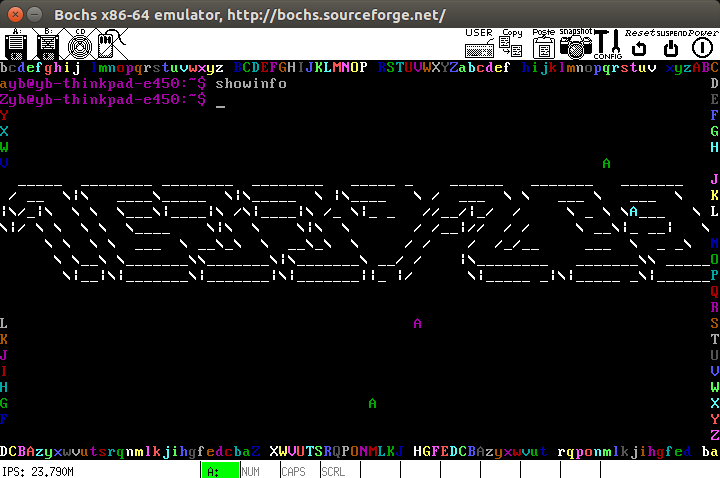
\includegraphics[scale=0.5]{assets/int_still_work.png}
        \caption{用于证明系统调用仍能正常执行的例子\label{fig:null}} 
        \end{center} 
    \end{figure} 
    
\section{实验总结}
    \subsection{亮点介绍}
    \subsubsection{方便的终端操控}
    本实验提供了新的终端指令。run stoneQ(或把stoneQ替换为stoneW,stoneA, stoneS)可以产生4种不同的用户程序进程。pc指令可以
    列出当前存在的所有进程、进程id以及他们所在的物理内存地址。kill <pid>命令可以杀死进程。clear命令可以做清屏。\\ 

    本实验创新地采用了如下的实现:在用户程序运行时,不退出终端。于是可以一边观察用户程序的执行,一边通过终端的操作增添或删除进程。
    这种交互性设计可以良好地检验出程序的正确性。用户只要乐意,可以创建任意多个进程,进程的代码段可以来自于四个用户程序中的任何一个。
    \subsubsection{内存分配器}
    本项目实现了内存分配。在运行一个新的用户程序时,不是通过硬编码的方式决定其内存位置,而是由内存分配器分配一段未只用的内存。\\ 

    回收的内存可以重复使用。图\ref{fig:kp}展示了相关情况。在杀死一个进程后,产生一个新的进程时,被回收的内存又被重新分配出去了。\\ 

    内存分配器的优点还在于,它允许了同一个用户程序被运行多次,例如图\ref{fig:3_stoneS}显示了相关情况。图中,同时运行了3个stoneS
    程序,这3个程序不分享内存地址,互不干扰地在独立的内存中执行。
    \subsubsection{与文件系统的配合}
    由于以前的项目实现了文件系统,本项目又实现了内存分配器,两者可以配合工作,发挥最大的作用。\\ 

    进程产生时,先通过内存分配器分配内存,再通过文件系统将文件载入到指定的内存空间中,再通过进程调度让进程自动执行。全程自动化程度高,
    程序灵活。

    \subsection{实验心得}
    这个实验表面上看很简单,但我还是花费了比较多的时间。而且上两周的学习任务比较重,这次实验几乎是在舍友都睡着了的时间段写完的。\\ 

    首先是进程的保存和恢复。由于思路没有完全理清,这部分的代码我重构了两三次。这之间我反复纠结的细节有:sp该如何存储?存储何时的sp?sp
    和ss如何恢复?恢复后栈顶的位置变了怎么办?ds该合适恢复?恢复后所有访存操作的行为都会改变,怎么办?我甚至还一度认为,``将寄存器从
    栈上拷贝到PCB''和``从PCB拷贝到栈上''这两个操作是没有必要的。 \\ 

    这些问题单独出现的时候都不难解决。但当他们在进程保存和进程恢复时同时出现时,就会成为一个比较大的困难。因为我必须同时解决好全部的这些问题。
    最终我采取的方案是,sp存储的是``保存完所有寄存器后''的sp,用mov的方式把sp压入栈中。恢复进程时先恢复sp和ss到被恢复进程的栈顶。ds
    直接用pop恢复,并保证保存和恢复现场的全程不访问内存。我经过仔细的考虑(和代码的实践后)得出简论,栈和PCB之间的拷贝是必要的,不做拷贝总会
    出现各种各样的困难,导致实现变得很复杂。\\ 

    得出上述的思考只用几句话的时间,但这是我一个凌晨的试错换来的。在调试的期间还遇到上述提到的忘关中断的BUG。这些错误堆积起来,让这次
    实验的完成变得更加困难了。但经过这次实验我对进程切换的理解也更深刻了。\\ 

    这次实验还有很多不足。个人认为最大的不足在于,太多的过程没有被封装成系统调用。由于C程序是对段透明的,这导致了当一个进程的段不为0时,
    调用许多C程序时,一旦发生寻址等操作,就会产生错误。正确的解决办法是利用中断修改cs,把ds同步成cs,此时ds就被同步到正确的段中。当执行完
    相关的操作后,再恢复ds,离开中断。这样就可以让许多内核级的操作在段不为0的程序上运行。更进一步地,终端进程就可以脱离内核代码而独立存在。
    在本项目中,终端依旧只能作为一个程序和内核链接在一起。
    \subsection{细节上的更新}
    \subsubsection{sscanf的实现}
    本项目实现了sscanf的大部分操作。实现了\%s, \%d, \%x, \%c,等匹配操作。为终端指令的提取提供基石。
    \subsubsection{内核拓展}
    内核从预留24个扇区拓展到预留40个扇区。修改了文件系统的相关配置。
    \subsubsection{文件系统的跨段处理}
    由于本次实验出现了跨段问题,而这在前几次项目中没有出现,故本项目略微修改了文件系统的实现,使其支持跨段的载入。
    \subsection{BUG汇总}\label{sec:bug}
    \subsubsection{文件系统的历史遗留问题}
    我的文件系统调用在传参时,某处地址的类型声明为了int16\_t。在之前这不会发生错误,因为以0x00为段寄存器时,偏移量最多为
    0xFFFF,在int16\_t的范围内。但是本项目发生了跨段,当我传入更高的地址时,会被int16\_t类型截断。导致程序无法载入到内存
    中。\\ 

    这个错误花费了比较多的时间。因为我的文件系统的结构化做得比较好,这也意味着函数调用会比较深。错误的追踪也比较困难。
    \subsubsection{中断未关闭的错误}
    在项目实现到一半时,我发现程序会卡死,而且时钟中断没有触发。这极其令人费解,我刚开始考虑了很多的情况,都没有找到这个问题发生的
    原因。我很疑惑为何时钟中断没有被触发。我试过手动往中断端口中写入数据允许下一次中断,确保硬件得到允许中断的信号。我使用手动调用
    int 08H,观察程序执行状态,发现程序正常执行,且栈能回到正确的位置。由于此时我已经写好了进程切换(正在测试中),我试过反复注释掉
    不同地方的代码观察情况。结果发现无论怎么改变代码,总有各种不同的错误。\\ 

    在折腾了很久后,突然有一个瞬间想到中断的问题。在内核初始化过程中关中断。在所有初始化结束后开中断。于是bug解决。\\ 

    我现在并没有完全弄懂为何这个BUG会导致时钟中断不再发生。毕竟时钟中断可能发生在程序执行的任何时刻,未关中断这个错误可能导致程序执行
    的任何一个时刻出错。分析出具体的原因太难了。但可以得知的是,不正确地开关中断是很严重的错误。
\begin{appendices}
\section{参考文献} \label{sec:reference}
\begin{enumerate}
    \item https://blog.csdn.net/longintchar/article/details/50602851 \\
    16位和32位汇编指令的不同(尤其是push指令)
    \item https://www.ibiblio.org/gferg/ldp/GCC-Inline-Assembly-HOWTO.html\#s1 \\
    GCC 内嵌汇编的书写。
  \end{enumerate}
\end{appendices}
\end{document}
